\chapter{Results}
\label{cha:results}

\newcolumntype{C}{>{\centering\arraybackslash}X}


\section{Experiment 1}
\textbf{Conditions:} L$f_{1}$R$\varnothing$ vs. L$f_{1}$R$f_{1}$ vs. L$\varnothing$R$f_{1}$; ($f_{1}$ = 7.5 Hz)\\ 

\subsection{RQ: Can we differentiate hemisphere-specific SSVEP responses based on the visually stimulated eye?}

\begin{table}[b]
\centering
\begin{tabularx}{\linewidth}{l *{6}{c}}
    \toprule
    \textbf{Compared} & \multicolumn{2}{c}{\textbf{Left}} & \multicolumn{2}{c}{\textbf{Middle}} & \multicolumn{2}{c}{\textbf{Right}} \\
    \textbf{Conditions} & \textbf{p(PO3)} & \textbf{p(O1)} & \textbf{p(POz)} & \textbf{p(Oz)} & \textbf{p(PO4)} & \textbf{p(O2)} \\
    \midrule
    L$f_{1}$R$\varnothing$ vs. L$f_{1}$R$f_{1}$ & 0.02 & <0.01 & 0.11 & 0.36 & 0.15 & 0.90 \\
    L$f_{1}$R$\varnothing$ vs. L$\varnothing$R$f_{1}$  & 0.02 & <0.01 & 0.79 & 0.28 & 0.41 & \textit{<0.01} \\
    L$f_{1}$R$f_{1}$ vs. L$\varnothing$R$f_{1}$ & 0.99 & 0.39 & 0.18 & 0.04 & 0.02 & <0.01 \\
    \bottomrule
\end{tabularx}
\caption{Experiment 1: Wilcoxon Test p-values for Amplitudes at 7.5 Hz.}
\label{tab:ex1-comparison_pvalues}
\end{table}


The table in \autoref{tab:ex1-comparison_pvalues} displays the outcomes of Wilcoxon tests conducted on SSVEP response amplitudes at a frequency of 7.5 Hz. The aim is to determine whether these response amplitudes differ based on the stimulated eye; the null hypothesis being \textit{"There is no difference in SSVEP responses or hemisphere-specific activity regardless of which eye is stimulated."} A low p-value in the lateral channels indicates strong evidence against the null hypothesis, suggesting a significant difference. Conversely, a higher p-value is expected for channels from the hemispheres that were stimulated in both cases.

The results lead to the following conclusions:

\begin{enumerate}
    \item \textbf{Stimulation Comparison 1: Left Eye vs. Both Eyes:}
    The p-values for the Left vs. Both comparison are 0.023 and $<0.001$ for p(PO3) and p(O1) respectively. As both p-values are less than the predefined significance level of 0.05, it can be inferred that significant disparities exist in SSVEP response amplitudes between the Left and Both conditions for channels PO3 and O1.
    
    \item \textbf{Stimulation Comparison 2: Left Eye vs. Right Eyes:}
    The p-values for the Left vs. Right comparison are 0.002 and $<0.001$ for p(PO3) and p(O1) respectively. Similarly, for channel pairs p(PO4) and p(O2), the p-values are 0.414 and $<0.001$ respectively. In all these cases, the p-values fall below 0.05, indicating significant discrepancies in SSVEP response amplitudes between the Left and Right conditions for these channels.
    
    \item \textbf{Stimulation Comparison 3: Both Eyes vs. Right Eyes:}
    The p-values for the Both vs. Right comparison are 0.022 and $<0.001$ for p(PO4) and p(O2) respectively. Once again, the p-values are lower than 0.05, indicating notable differences in SSVEP response amplitudes between the Both and Right conditions for these channels.
\end{enumerate}

In summary, the results from the Wilcoxon tests suggest the presence of statistically significant evidence against the null hypothesis.


\begin{figure}[hb]
    \centering
    
    \begin{subfigure}{1.0\textwidth}
        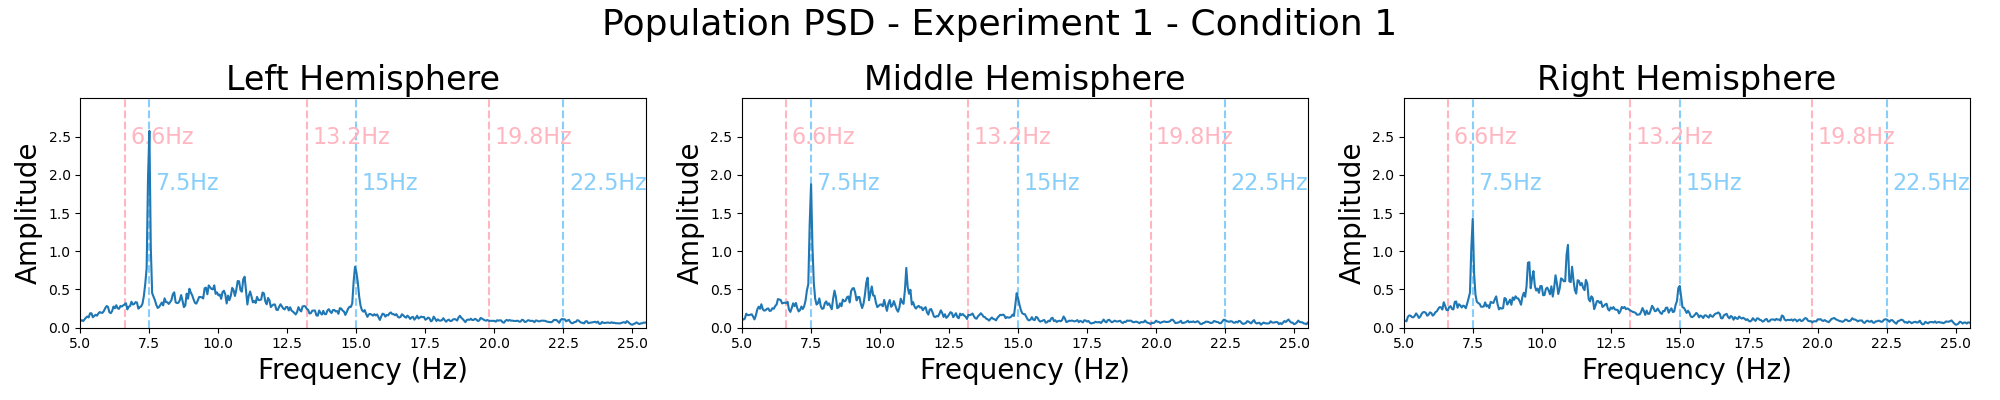
\includegraphics[width=\linewidth]{images/results/e100.png}
        \caption{Condition 1: L$f_{1}$R$\varnothing$}
        \label{fig:e100}
    \end{subfigure}
    
    \begin{subfigure}{1.0\textwidth}
        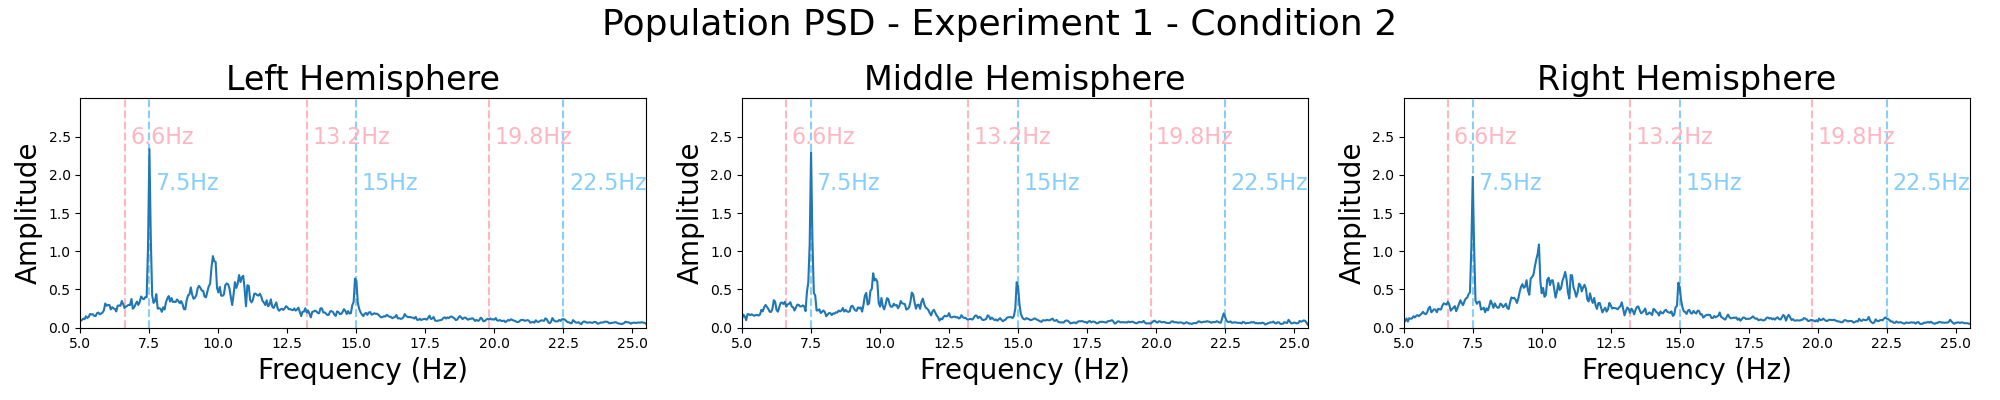
\includegraphics[width=\linewidth]{images/results/e101.png}
        \caption{Condition 2: L$f_{1}$R$f_{1}$}
        \label{fig:e101}
    \end{subfigure}
    
    \begin{subfigure}{1.0\textwidth}
        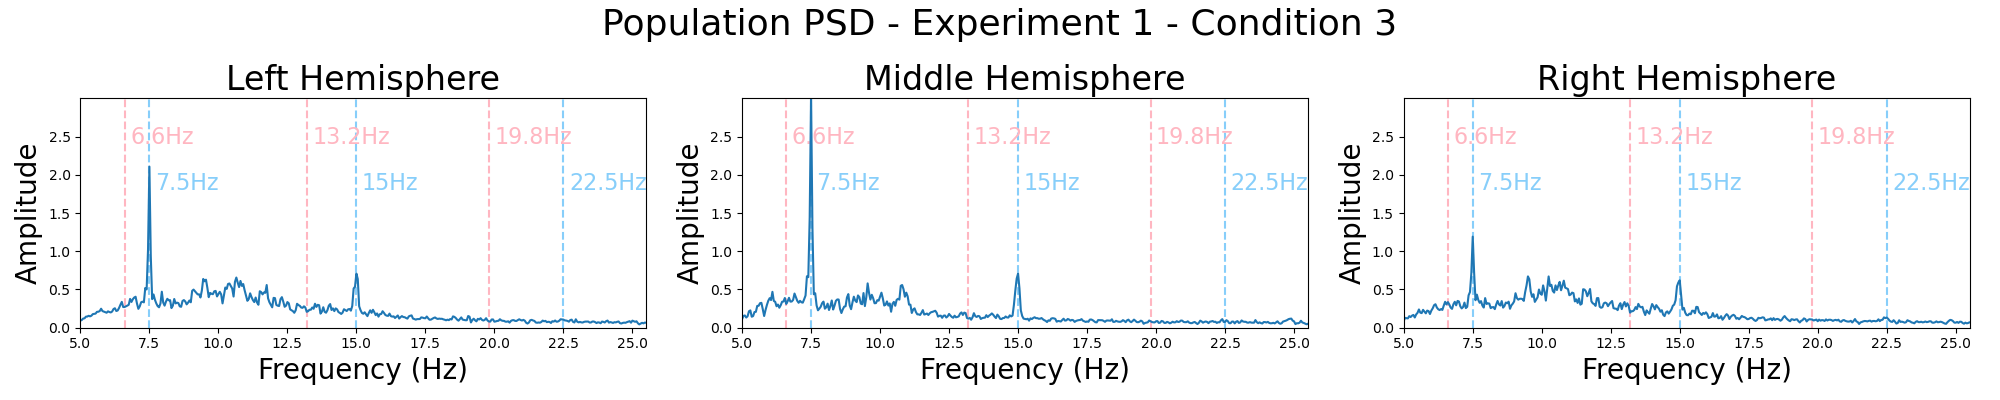
\includegraphics[width=\linewidth]{images/results/e102.png}
        \caption{Condition 3: L$\varnothing$R$f_{1}$}
        \label{fig:e102}
    \end{subfigure}
    \caption{Experiment 1: Population PSD Analysis.}
    \emph{Note: The y-axis is twice the height of the y-axes in the other experiments.}

    \label{fig:e1_population}
\end{figure}







\clearpage


\section{Experiment 2}
\textbf{Conditions:}  L$f_{1}$R$f_{2}$ vs. L$f_{2}$R$f_{2}$  vs. L$f_{2}$R$f_{1}$; ($f_{1}$ = 7.5 Hz, $f_{2}$ = 6.6 Hz)\\ 

\subsection{RQ: Can we differentiate SSVEP responses based on the unique frequency stimuli presented to each eye?}


In Tables \ref{tab:ex2-66}, \ref{tab:ex2-75} the amplitudes of the signals at $f_{2}$ and $f_{1}$ are compared respectively. In table \ref{tab:ex2-ratios} the ratio of the amplitude($f_{1}$)/amplitude($f_{2}$) is calculated per signal and then compared. The statistical comparisons is done using the Wilcoxon method.

We observe low p-values in the cases where one of the compared signals is mono SSVEP (e.g. L$f_{1}$R$f_{1}$ or L$f_{2}$R$f_{2}$). In previous Figures \ref{fig:e1_population} and \ref{fig:e111} it is seen that the amplitude in mono SSVEP is usually double or more that of dual-SSVEP. 

Interesting are the L$f_{1}$R$f_{2}$ vs. L$f_{2}$R$f_{1}$ comparisons in the tables. In Table \ref{tab:ex2-66} the p-values in the lateral PO3, PO4, O2 channels are shown in to be low; in Table \ref{tab:ex2-75} the same is true only for the O1 channel. This shows some, but not strong, evidence against the null hypothesis of \textit{"SSVEP responses cannot be differentiated based on the unique frequency stimuli presented to each eye"}, in the cases where two different frequencies are used.






\begin{table}[ht]
\centering
\begin{tabularx}{\linewidth}{l *{6}{c}}
    \toprule
    \textbf{Compared} & \multicolumn{2}{c}{\textbf{Left}} & \multicolumn{2}{c}{\textbf{Middle}} & \multicolumn{2}{c}{\textbf{Right}} \\
    \textbf{Conditions} & \textbf{p(PO3)} & \textbf{p(O1)} & \textbf{p(POz)} & \textbf{p(Oz)} & \textbf{p(PO4)} & \textbf{p(O2)} \\
    \midrule
    L$f_{1}$R$f_{1}$ vs. L$f_{1}$R$f_{2}$ & <0.01 & <0.01 & 0.03 & <0.01 & 0.21 & <0.01 \\
    L$f_{1}$R$f_{1}$ vs. L$f_{2}$R$f_{2}$ & <0.01 & <0.01 & <0.01 & <0.01 & <0.01 & <0.01 \\
    L$f_{1}$R$f_{1}$ vs. L$f_{2}$R$f_{1}$ & 0.04 & <0.01 & 0.15 & 0.11 & 0.09 & 0.20 \\
    L$f_{1}$R$f_{2}$ vs. L$f_{2}$R$f_{2}$ & <0.01 & 0.14 & 0.03 & <0.01 & <0.01 & <0.01 \\
    L$f_{1}$R$f_{2}$ vs. L$f_{2}$R$f_{1}$ & 0.01 & 0.83 & 0.55 & <0.01 & 0.53 & 0.06 \\
    L$f_{2}$R$f_{2}$ vs. L$f_{2}$R$f_{1}$ & <0.01 & 0.08 & <0.01 & <0.01 & <0.01 & <0.01 \\
    \bottomrule
\end{tabularx}
\caption{Experiment 2: Wilcoxon Test p-values for Amplitudes at 6.6 Hz.}
\label{tab:ex2-66}
\end{table}


\begin{table}[ht]
\centering
\begin{tabularx}{\linewidth}{l *{6}{c}}
    \toprule
    \textbf{Compared} & \multicolumn{2}{c}{\textbf{Left}} & \multicolumn{2}{c}{\textbf{Middle}} & \multicolumn{2}{c}{\textbf{Right}} \\
    \textbf{Conditions} & \textbf{p(PO3)} & \textbf{p(O1)} & \textbf{p(POz)} & \textbf{p(Oz)} & \textbf{p(PO4)} & \textbf{p(O2)} \\
    \midrule
    L$f_{1}$R$f_{1}$ vs. L$f_{1}$R$f_{2}$ & <0.01 & <0.01 & <0.01 & <0.01 & <0.01 & <0.01 \\
    L$f_{1}$R$f_{1}$ vs. L$f_{2}$R$f_{2}$ & <0.01 & <0.01 & <0.01 & <0.01 & <0.01 & <0.01 \\
    L$f_{1}$R$f_{1}$ vs. L$f_{2}$R$f_{1}$ & <0.01 & <0.01 & <0.01 & <0.01 & <0.01 & <0.01 \\
    L$f_{1}$R$f_{2}$ vs. L$f_{2}$R$f_{2}$ & <0.01 & <0.01 & 0.08 & <0.01 & <0.01 & <0.01 \\
    L$f_{1}$R$f_{2}$ vs. L$f_{2}$R$f_{1}$ & 0.28 & 0.01 & 0.85 & 0.19 & 0.16 & 0.24 \\
    L$f_{2}$R$f_{2}$ vs. L$f_{2}$R$f_{1}$ & 0.01 & 0.17 & 0.07 & <0.01 & 0.01 & 0.03 \\
    \bottomrule
\end{tabularx}
\caption{Experiment 2: Wilcoxon Test p-values for Amplitudes at 7.5 Hz.}
\label{tab:ex2-75}
\end{table}



\begin{table}[ht]
\centering
\begin{tabularx}{\linewidth}{l *{6}{c}}
    \toprule
    \textbf{Compared} & \multicolumn{2}{c}{\textbf{Left}} & \multicolumn{2}{c}{\textbf{Middle}} & \multicolumn{2}{c}{\textbf{Right}} \\
    \textbf{Conditions} & \textbf{p(PO3)} & \textbf{p(O1)} & \textbf{p(POz)} & \textbf{p(Oz)} & \textbf{p(PO4)} & \textbf{p(O2)} \\
    \midrule
    L$f_{1}$R$f_{1}$ vs. L$f_{1}$R$f_{2}$ & <0.01 & <0.01 & <0.01 & <0.01 & 0.01 & <0.01 \\
    L$f_{1}$R$f_{1}$ vs. L$f_{2}$R$f_{2}$ & <0.01 & <0.01 & <0.01 & <0.01 & <0.01 & <0.01 \\
    L$f_{1}$R$f_{1}$ vs. L$f_{2}$R$f_{1}$ & <0.01 & <0.01 & <0.01 & <0.01 & <0.01 & <0.01 \\
    L$f_{1}$R$f_{2}$ vs. L$f_{2}$R$f_{2}$ & <0.01 & <0.01 & 0.01 & <0.01 & <0.01 & <0.01 \\
    L$f_{1}$R$f_{2}$ vs. L$f_{2}$R$f_{1}$ & 0.75 & 0.21 & 0.81 & <0.01 & 0.19 & 0.90 \\
    L$f_{2}$R$f_{2}$ vs. L$f_{2}$R$f_{1}$ & <0.01 & 0.01 & <0.01 & <0.01 & <0.01 & <0.01 \\
    \bottomrule
\end{tabularx}
\caption{Experiment 2: Wilcoxon Test p-values for ratio of Amplitudes 6.6 Hz / 7.5 Hz.}
\label{tab:ex2-ratios}
\end{table}


\subsection{RQ: Can we simultaneously elicit separate SSVEP responses in both hemispheres?}
% Separate SSVEP responses cannot be simultaneously elicited in both hemispheres. \\


In the Population PSD Figure \ref{fig:e2_population}, distinct amplitude peaks are observable for the dual stimulating frequencies, 7.5 Hz and 6.6 Hz, indicating the presence of dual-SSVEP responses.

For the specific frequencies, where $f_{1}$ is 7.5 Hz and $f_{2}$ is 6.6 Hz, the patterns in amplitude responses are notable in different conditions as shown in the following figures:

In Figure \ref{fig:e110} (L$f_{1}$R$f_{2}$), it's evident that generally, the amplitude of the 6.6 Hz frequency is lower than that of 7.5 Hz in both the left and right hemispheres. Notably, in the left hemisphere, the amplitude of 6.6 Hz is higher than that in the right hemisphere, which is consistent with the simulation being presented to the right eye.

Moving to Figure \ref{fig:e111} (L$f_{2}$R$f_{2}$), during mono SSVEP stimulation, the 6.6 Hz frequency exhibits a considerably higher SSVEP response, being twice as high as other frequencies. This trend echoes that observed in Figure \ref{fig:e1_population}.

Lastly, Figure \ref{fig:e112} (L$f_{2}$R$f_{1}$) reveals that the amplitude of 6.6 Hz is higher than that of 7.5 Hz in both the left and right hemispheres. However, at 7.5 Hz, the amplitude is higher in the right hemisphere compared to the left. Notably, the amplitude of 6.6 Hz is greater in the left hemisphere than in the right, underscoring a frequency-specific asymmetry.


\begin{figure}[h]
    \centering
    
    \begin{subfigure}{1.0\textwidth}
        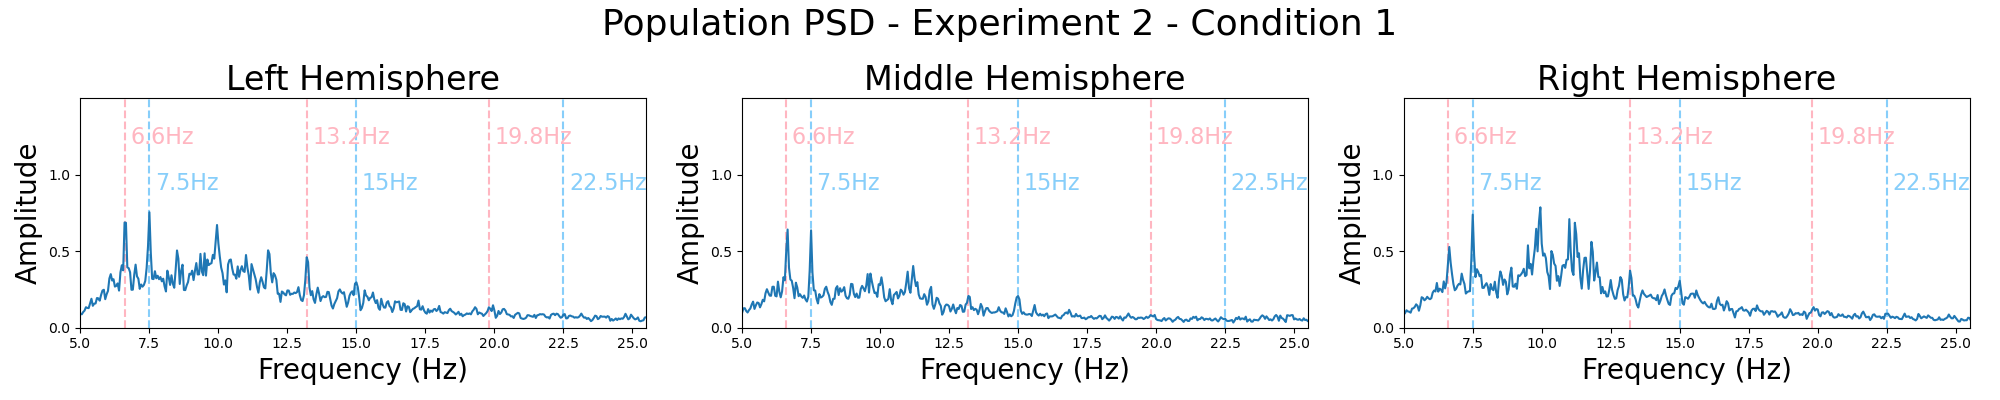
\includegraphics[width=\linewidth]{images/results/e110.png}
        \caption{Condition 1: L$f_{1}$R$f_{2}$}
        \label{fig:e110}
    \end{subfigure}
    

    \begin{subfigure}{1.0\textwidth}
        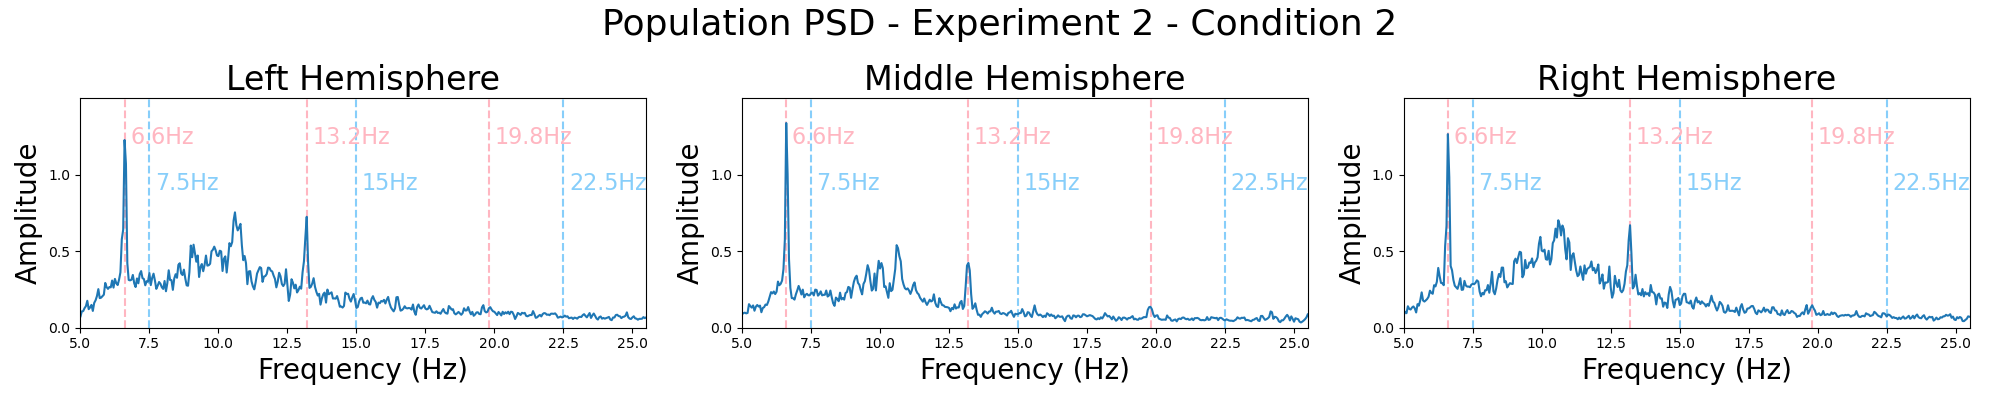
\includegraphics[width=\linewidth]{images/results/e111.png}
        \caption{Condition 2: L$f_{2}$R$f_{2}$}
        \label{fig:e111}
    \end{subfigure}
    
    \begin{subfigure}{1.0\textwidth}
        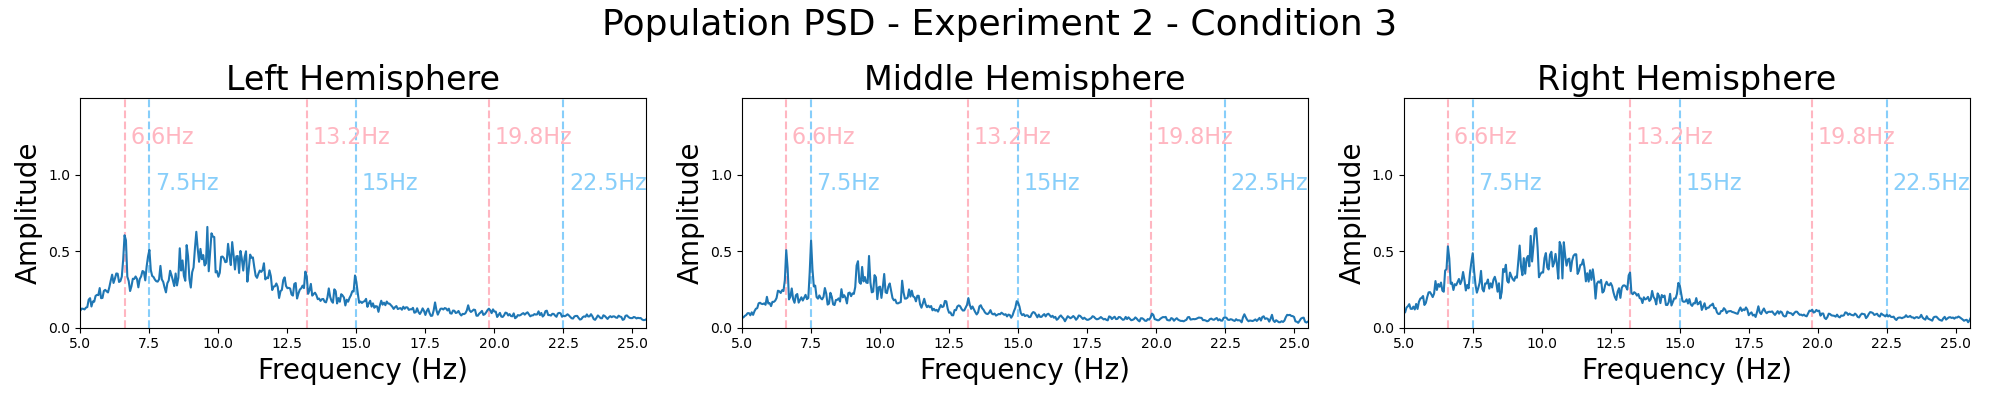
\includegraphics[width=\linewidth]{images/results/e112.png}
        \caption{Condition 3: L$f_{2}$R$f_{1}$}
        \label{fig:e112}
    \end{subfigure}
    
    \caption{Experiment 2: Population PSD Analysis}
    \label{fig:e2_population}
\end{figure}


\clearpage
\section{Experiment 3}
\textbf{Conditions:} BR-L$f_{2}$R$f_{1}$ \\

The experiment aimed to determine whether binocular rivalry could be achieved in a virtual reality environment. All participating individuals consistently reported experiencing binocular rivalry during the course of the experiment.

\begin{figure}[h]
    \centering
    
    \begin{subfigure}{1.0\textwidth}
        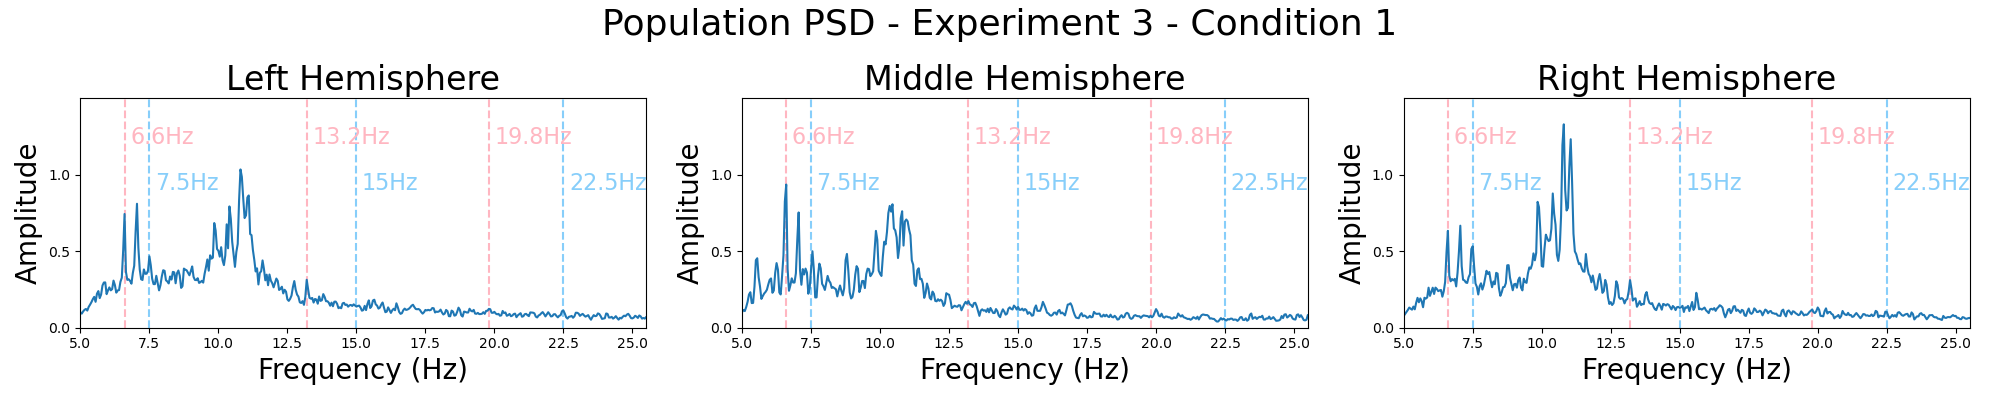
\includegraphics[width=\linewidth]{images/results/e120.png}
        \caption{Condition 1: BR L$f_{2}$,~R$f_{1}$ (BR)}
        \label{fig:e120}
    \end{subfigure}
    \caption{Experiment 3: Population PSD Analysis}
    \label{fig:e3_population}
\end{figure}

While not originally a part of our research questions, we conducted a statistical t-test on the signals to assess hemisphere separation.

The EEG signal underwent segmentation into left, middle, and right hemispheres, and signal strengths at 6.6 Hz and 7.5 Hz were measured. Their ratio was calculated and subjected to testing.

The outcomes of our statistical evaluation are noteworthy. The p-value for the comparison between the Left and Middle hemispheres yielded a relatively high value of 0.915, indicating a lack of substantial difference between these regions. Comparably, the p-value for the Left vs. Right comparison was 0.061, implying a possible discrepancy in strengths. This trend persisted in the Middle vs. Right comparison with a p-value of 0.055.

Although these p-values hover around the conventional significance threshold of 0.05, they do not provide conclusive evidence to reject the null hypothesis, which posits no hemisphere separation.

Of particular interest is the distinct peak observed around 7 Hz in the Population PSD Figure \ref{fig:e3_population}. Remarkably, this distinctive feature was absent in other experimental conditions. Moreover, we noted a heightened presence of noise in the alpha wave range (8–12 Hz).

\begin{table}[h]
\centering
\begin{tabular}{c *{3}{>{\centering\arraybackslash}m{2cm}}}
\toprule
\textbf{Hemisphere Comparison} & \textbf{p-value} \\
\midrule
Left vs. Middle & 0.915 \\
Left vs. Right & 0.061 \\
Middle vs. Right & 0.055 \\
\bottomrule
\end{tabular}
\caption{Experiment 3: T-Test Analysis of p-values for Different Hemispheres.}
\label{tab:pvalues}
\end{table}






\clearpage
\section{Experiment 4}
\textbf{Conditions:} FL-BR-L$f_{2}$R$f_{1}$ vs.  FR-BR-L$f_{2}$R$f_{1}$ \\


\subsection{RQ: Can the direction of participants' attention control or influence binocular rivalry?}

Figure \ref{fig:e4_population} illustrates the Population PSD. A distinct disparity becomes apparent when comparing two scenarios: in the "Focus Right" condition (Figure \ref{fig:e131}), a prominent peak at 7.5 Hz is observable in both hemispheres, accompanied by attenuation of the 6.6 Hz frequency. This stands in contrast to the "Focus Left" scenario (Figure \ref{fig:e130}). These findings present compelling indications that binocular rivalry might be controllable.

The analysis of Tables \ref{tab:ex4-p66}, \ref{tab:ex4-p75}, and \ref{tab:ex4-p66/75} reveals notable statistical distinctions primarily within the PO3, POz, Oz, and O2 channels. However, these differences do not reach a level of statistical significance to refute the null hypothesis.

\begin{figure}[b]
    \centering
    
    \begin{subfigure}{1.0\textwidth}
        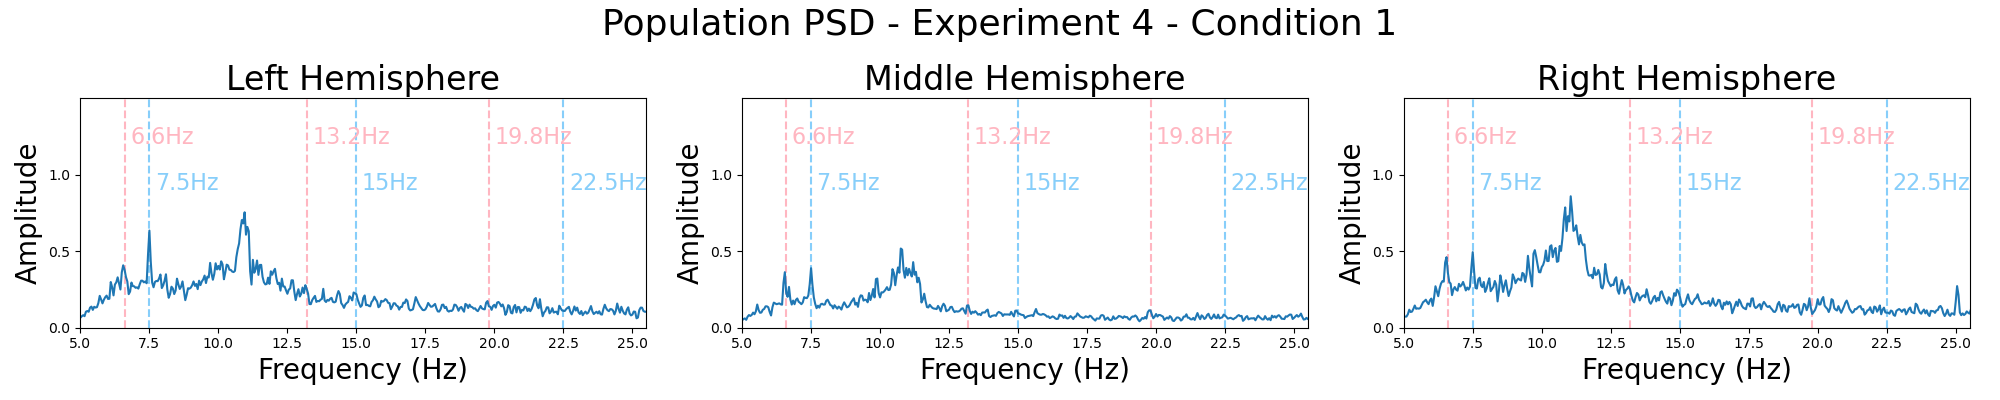
\includegraphics[width=\linewidth]{images/results/e130.png}
        \caption{Condition 1: Focus Left - BR L$f_{2}$,~R$f_{1}$ (FL-BR)}
        \label{fig:e130}
    \end{subfigure}
    
    \begin{subfigure}{1.0\textwidth}
        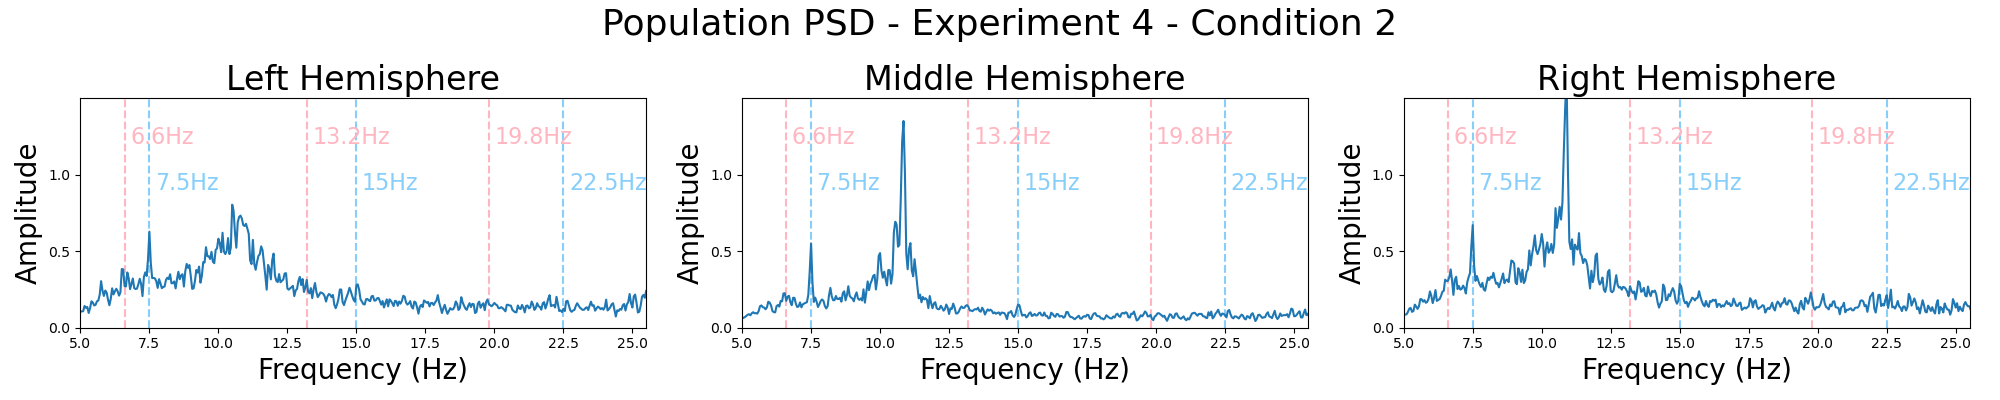
\includegraphics[width=\linewidth]{images/results/e131.png}
        \caption{Condition 2: Focus Right - BR L$f_{2}$,~R$f_{1}$ (FR-BR)}
        \label{fig:e131}
    \end{subfigure}
    
    \caption{Experiment 4: Population PSD Analysis}
    \label{fig:e4_population}
\end{figure}




\begin{table}[b]
\centering
\begin{tabularx}{\linewidth}{l *{6}{c}}
    \toprule
    \textbf{Comparison} & \multicolumn{2}{c}{\textbf{Left}} & \multicolumn{2}{c}{\textbf{Middle}} & \multicolumn{2}{c}{\textbf{Right}} \\
     \textbf{Conditions}& \textbf{p(PO3)} & \textbf{p(O1)} & \textbf{p(POz)} & \textbf{p(Oz)} & \textbf{p(PO4)} & \textbf{p(O2)} \\
    \midrule
    BR vs. FL-BR & 0.03 & 0.97 & 0.45 & 0.27 & 0.88 & 0.22 \\
    BR vs. FR-BR & 0.01 & 0.98 & 0.13 & <0.01 & 0.21 & 0.40 \\
    FL-BR vs. FR-BR & 0.48 & 0.64 & 0.41 & 0.06 & 0.44 & 0.14 \\
    \bottomrule
\end{tabularx}
\caption{Experiment 4: Wilcoxon Test p-values for ratio of Amplitudes 6.6 Hz / 7.5 Hz.}
\label{tab:ex4-p66/75}
\end{table}


\begin{table}[t]
\centering
\begin{tabularx}{\linewidth}{l *{6}{c}}
    \toprule
    \textbf{Comparison} & \multicolumn{2}{c}{\textbf{Left}} & \multicolumn{2}{c}{\textbf{Middle}} & \multicolumn{2}{c}{\textbf{Right}} \\
    \textbf{Conditions} & \textbf{p(PO3)} & \textbf{p(O1)} & \textbf{p(POz)} & \textbf{p(Oz)} & \textbf{p(PO4)} & \textbf{p(O2)} \\
    \midrule
    BR vs. FL-BR & 0.06 & 0.28 & 0.07 & 0.02 & 0.71 & 0.20 \\
    BR vs. FR-BR & 0.02 & 0.63 & 0.64 & <0.01 & 0.03 & 0.18 \\
    FL-BR vs. FR-BR & 0.77 & 0.37 & 0.24 & 0.16 & 0.04 & 0.91 \\
    \bottomrule
\end{tabularx}
\caption{Experiment 4: Wilcoxon Test p-values for Amplitudes at 7.5 Hz.}
\label{tab:ex4-p75}
\end{table}


\begin{table}[t]
\centering
\begin{tabularx}{\linewidth}{l *{6}{c}}
    \toprule
    \textbf{Comparison } & \multicolumn{2}{c}{\textbf{Left}} & \multicolumn{2}{c}{\textbf{Middle}} & \multicolumn{2}{c}{\textbf{Right}} \\
    \textbf{Conditions}& \textbf{p(PO3)} & \textbf{p(O1)} & \textbf{p(POz)} & \textbf{p(Oz)} & \textbf{p(PO4)} & \textbf{p(O2)} \\
    \midrule
    BR vs. FL-BR & 0.65 & 0.23 & 0.05 & 0.40 & 0.88 & 0.47 \\
    BR vs. FR-BR & 0.04 & 0.10 & <0.01 & 0.04 & 0.83 & 0.07 \\
    FL-BR vs. FR-BR & 0.06 & 0.91 & 0.19 & 0.11 & 0.99 & 0.01 \\
    \bottomrule
\end{tabularx}
\caption{Experiment 4: Wilcoxon Test p-values for Amplitudes at 6.6 Hz.}
\label{tab:ex4-p66}
\end{table}
